
In order to illustrate our vision, let us consider an example from the domain of energy
management. We assume we are interested in queries like: \textit{Give a list
of energy providers that can provision 1000 KW-h, in the next 10 seconds, that are close to my city, with a cost of 0,50 Euro/KW-h and that are labeled as green?} We consider a simplified SLA cloud contract inspired in the cheapest contract provided by Azure: \textit{cost of \$0,05 cents per call,  8~GB of I/O volume/month, free data transfer cost within the same region,  1~GB of storage.} 
Suppose that the user is ready to pay a maximum of \textit{\$5 as total query cost}; she requests that only  \textit{green} energy providers should be  listed (provenance), with at least  \textit{85$\%$} of precision of provided data, even if they are not fresh; she requires an availability rate of at least 90$\%$ and a response time of  \textit{0,01 s}. 
  The question is how can the user efficiently obtain  results for her queries such that they meet her QoS requirements, they respect her subscribed contracts with the involved cloud provider(s) and such that they do not neglect services contracts? 

According to our classification scheme that resulted from our systematic mapping, we propose a new vision of data integration. This vision includes the description of the context in which data integration is done in modern environments. It also identifies the phases of the data integration process with its associated problems and challenges when they must include SLAs and QoS preferences expressed by data consumers. 


\subsection{Data integration context}
We consider that data integration is done under new conditions with respect to type of data sources, the environment where it is performed and the preferences  of data consumers and the SLA. We assume that data integration is done on a (multi)-cloud service oriented environment shown in Figure \ref{fig:vision}. 
\begin{figure}[h!]
\centering
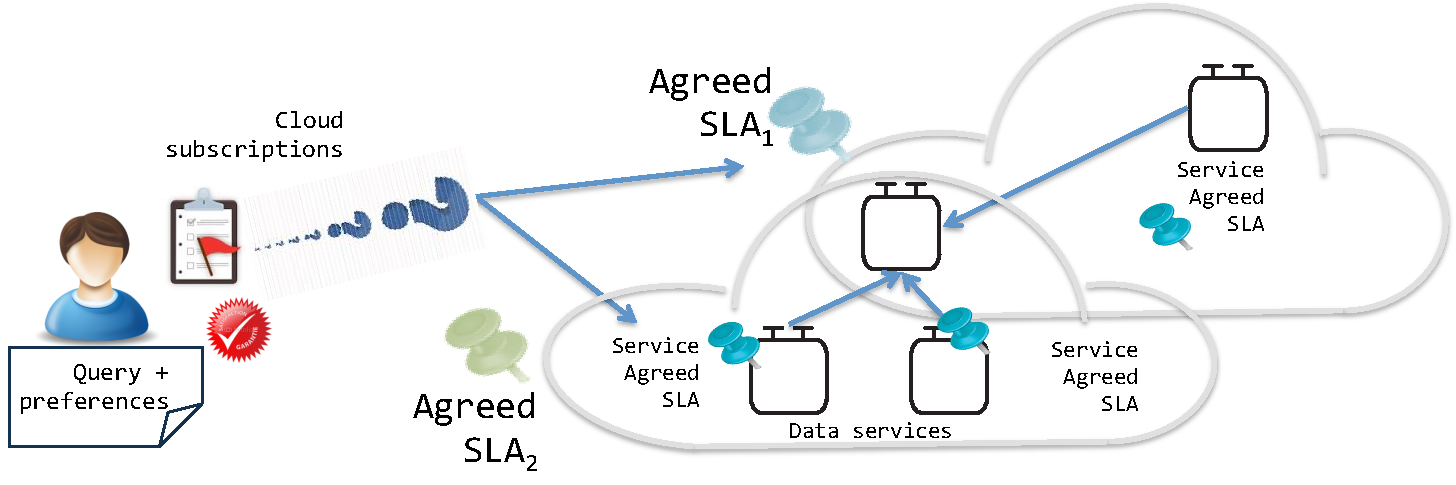
\includegraphics[scale=0.50]{figs/DataIntegrationContext.pdf} 
\caption{New data integration context}\label{fig:vision}
\end{figure}

There are data providers that are services possibly deployed in clouds and available  through their API or in a REST architecture. We assume that  each service exports an agreed SLA that specifies the economic cost per call, the maximum number of calls that can be done per day, the availability of the service, the average response time when a method is called, the reliability, the privacy of the produced data (whether they can be stored or not), the precision of their responses, freshness and provenance of the produced data.  

%\begin{trivlist}\sf\footnotesize
%\item[~$\bullet$ ] {\sf agreedSLA:$\langle$cost/call, maxCalls/day, availability, responseTime, reliability, privacy, precision, freshness, provenance$\rangle$}. 
 %\end{trivlist}


Cloud providers define also their SLA contracts expressing  subscription contracts that specify, the cost per request ({\sf cost/request}), the volume of data that can be exchanged per month ({\sf I/0 volume/month}), the cost of transferring data or applications within the same data centre or between data centres ({\sf datatransferCost/region}), and storage space ({\sf storageSpace}). For example some cloud providers enable the customer to choose the zone to install PaaS services and deploy applications (e.g. zone 1 is Europe). If the customer wishes to deploy services in zone 1 but store data in zone 2 the transfer cost will change.

%\begin{trivlist}\sf\footnotesize
 %\item[~$\bullet$ ]  {\sf cloudSLA:$\langle$cost/request, I/0 volume/month, datatransferCost/region, storageSpace$\rangle$}. 
 %\end{trivlist}


Some of these measures ({\sf cost/call, maxCall/day}) are static and explicitly specified by the service provider. 
In contrast, the other measures should be computed by monitoring the conversations between the service and the applications that contact it.  

In our vision a query expressed in an SQL-like language is associated to a set of QoS preferences expressing the requirements of the user. For example, the economic cost she is ready to pay for executing the query, the provenance of the data, the reputation of data services and the expected time response. The answer of such a query is the result of integrating data from different services according to a series of phases described in the following section.

\subsection{SLA guided data integration}
Thus, given a query, its associated QoS preferences, cloud providers  and  services that can potentially be data providers (see Figure \ref{fig:vision}),  SLA guided data  integration can consist in four steps.  
%\begin{itemize}
\paragraph{Generating a derived SLA}  
The key and original aspect of   our proposed data integration and provision process is  to define  a vertical mapping of user QoS preferences and agreed SLAs. This  leads to a {\em derived SLA} that guides the evaluation of a query. 

A query has associated preferences  expressed as macroscopic constraints (i.e. user preferences statement): execution time, pay / no pay, data reliability, provenance, freshness, privacy, partial/full results, delivery mode. These constraints are coupled with the profile of the user which is in general stated in her cloud subscription (amount of assigned storage space, number of requests, I/O transferred Mega bytes, etc.). 

Given agreed SLA's and a user preferences statement the challenge is to compute a  {\em derived SLA} that  maps SLA measures and preferences attributes.  The derived SLA is defined as a set of measures that correspond to the user preferences computed as a function of different static, computed and hybrid measures. The {\em derived SLA}  will guide the way the query will be evaluated, and the way results will be computed and delivered.
Therefore, we propose to classify SLA measures to represent the relationship between fine grained measures used by agreed SLAs and coarse grained measures used in user preferences statements. It is also necessary to specify how to compute coarse grained measures with fine grained ones. For example, data precision will be computed as a function of availability, freshness and provenance exported by data services. 

  
\paragraph{Filtering data services} 
The derived SLA  is used for filtering possible data services that can be used for answering the query. This is done using a set of matching algorithms based on  graph structures and RDF specifications. This step may lead either to the rejection of integration in case of total incompatibility, or to a negotiation between SLA which will lead us to the proposal for a negotiated SLA integration and thus the need for an adaptive setting.


\paragraph{Query rewriting} 
Given a set of data services that can potentially provide data for integrating the query result, we compute possible data service compositions that give partial or exhaustive  results according to the derived SLA and the agreed SLA of each data service. The objective is to   generate a number $k$ of service compositions, combining as much as possible the services available such that the constraints of the derived SLA are verified. 


\paragraph{Integrating a query result} 
The service compositions are executed in one or several clouds where the user has a subscription. The execution cost of  service compositions must fulfill the derived SLA (that expresses user requirements). In this phase we generate an execution plan  considering the derived SLA and the subscription of the user to one or several clouds. We consider for example the economic cost determined by the data to be transferred, the number of external calls to services, data storage and results delivery costs and we decide how to use clouds resources for executing the composition. A first approach for performing this phase has been addressed  in  \cite{Lopez14}.

The first phase is an open issue for dealing with SLAs and particularly for adding quality dimensions to  data integration. The problem is complex because SLA describe different elements participating in the data integration process: data services, cloud services at the different levels of the architecture (i.e., IaaS, PaaS, SaaS), data consumers subscriptions to cloud providers. The SLAs contain measures related to the way services are provided but also related to the data they provide. All these aspects must be considered for matching resources (i.e., services) with data consumers preferences. As shown in the following section and in our study SLA models and languages have been proposed. In contrast  efficient preferences and SLAs matching algorithms need to be proposed to compute derived SLAs. Concerning the other data integration phases, they have been partially addressed by existing works, where some quality dimensions are considered (e.g., data privacy). In our vision there are open issues to be addressed in order to have solutions that consider SLA in order to enhance data integration in multi-cloud environments. 

